\documentclass{article}%
\usepackage[T1]{fontenc}%
\usepackage[utf8]{inputenc}%
\usepackage{lmodern}%
\usepackage{textcomp}%
\usepackage{lastpage}%
\usepackage[head=40pt,margin=0.5in,bottom=0.6in]{geometry}%
\usepackage{graphicx}%
%
\title{\textbf{España accedió a extraditar al guardaespaldas de Chávez a Venezuela}}%
\author{EFE}%
\date{23/11/2018}%
%
\begin{document}%
\normalsize%
\maketitle%
\textbf{URL: }%
http://www.el{-}nacional.com/noticias/politica/espana{-}accedio{-}extraditar{-}guardaespaldas{-}chavez{-}venezuela\_260856\newline%
%
\textbf{Periodico: }%
EN, %
ID: %
260856, %
Seccion: %
Política\newline%
%
\textbf{Palabras Claves: }%
España, Política, Mundo\newline%
%
\textbf{Derecho: }%
CONTEXTO%
, Otros Derechos: %
1.10%
, Sub Derechos: %
1.10.1%
\newline%
%
\textbf{EP: }%
NO\newline%
\newline%
%
\textbf{\textit{Las autoridades del país europeo aseguran que Adrián Velásquez Figueroa no puede ser perseguido político debido a que es miembro de la administración de Chávez}}%
\newline%
\newline%
%
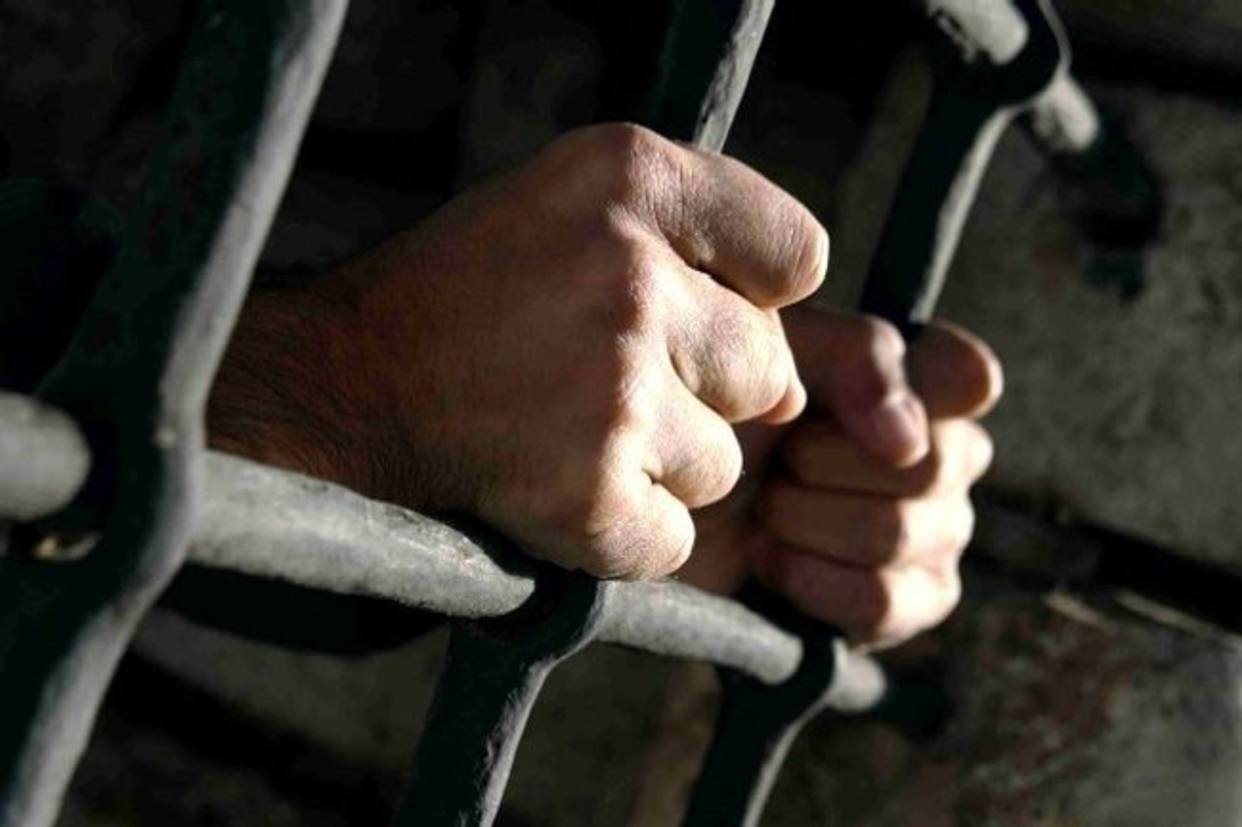
\includegraphics[width=300px]{63.jpg}%
\newline%
%
La Audiencia Nacional de España accedió este viernes a extraditar a Venezuela a Adrián Velásquez Figueroa, guardaespaldas y jefe de seguridad del presidente fallecido Hugo Chávez, al entender que no puede ser un perseguido político porque no es un opositor.%
\newline%
%
La Audiencia siguió así el mismo criterio que con la esposa de Velásquez, Claudia Patricia Díaz Guillén, reclamada también por Venezuela, quien ejerció durante años como enfermera de Chávez y fue detenida en Madrid junto a su esposo.%
\newline%
%
En el caso de Velásquez, el tribunal rechaza que pueda ser represaliado en Venezuela porque, según los jueces, no es un opositor sino un miembro de la administración de Chávez, y el actual gobierno de Nicolás Maduro "es continuista" con su línea.%
\newline%
%
El gobierno de Venezuela reclama a la pareja por delitos de blanqueo y enriquecimiento a raíz de la publicación de los Papeles de Panamá, en los que aparecen empresas relacionadas con Velásquez con las que, según las autoridades del país, lavaron dinero que sustrajeron de las arcas públicas.%
\newline%
%
La defensa de Velásquez alegó que era peligroso entregarlo al gobierno de Venezuela porque asegura que en el país se violan los derechos humanos constantemente.~También destacó la persecución que sufren los dirigentes de la oposición.%
\newline%
%
El tribunal español reconoció que el gobierno venezolano ha motivado el pronunciamiento por parte de organismos internacionales que denuncian la vulneración de derechos; sin embargo, señaló que la persecución política en la que se cometen las violaciones de los derechos humanos está orientada hacia la oposición.%
\newline%
%
Recordaron que Velásquez ocupó cargos relevantes como miembro de la Guardia de Honor de Chávez y estuvo en puestos cercanos Ejecutivo. Además, poco después de cesar en estos cargos en 2012~abandonó el país.%
\newline%
%
"Todo ello nos pone de manifiesto que el señor Velásquez no ha sufrido personalmente ninguna clase de persecución política, ni tampoco se presume que pueda sufrirla por el hecho de haber formado parte de la Dirección General de Contrainteligencia Militar (Dgcim)y de la Guardia de Honor Presidencial", afirmaron.%
\newline%
%
El tribunal cree que se cumplen los requisitos de doble incriminación, pero acota los delitos por los que se le podría condenar en España, que serían malversación o cohecho y blanqueo de capitales.%
\newline%
%
La esposa de Velásquez, que fue enfermera personal de Chávez y de 2011 a 2013 responsable del Tesoro de la nación, recurrió la decisión de la Audiencia Nacional de acceder a su extradición a Venezuela por los mismos motivos que su marido y anunció que pedirá asilo en España.%
\newline%
%
Díaz Guillén aseguró esta semana en una entrevista con Efe que las acusaciones contra ella y su esposo han sido fabricadas por las autoridades venezolanas.%
\newline%
%
\end{document}